%%%%%%%%%%%%%%%%%%%%%%%%%%%%%%%%%%%%%%%%%%%%%%%%%%%%%%%%%%%%%%%%%%%%%%%%%%%
%%  chapter1.tex  –  Chapter 1: Literature Review and Gap Analysis
%%  v9 – Restructured following progressive scope of the research:
%%       CT dynamics → distributed → efficiency → non-stationarity.
%%       Covers all 12 intersections of 3 conditions × 4 requirements.
%%       7 gaps identified. Bridging statements between sections.
%%       Only \section headings added to TOC.
%%%%%%%%%%%%%%%%%%%%%%%%%%%%%%%%%%%%%%%%%%%%%%%%%%%%%%%%%%%%%%%%%%%%%%%%%%%

\chapter{Analysis of Hybrid Intrusion Detection and Prevention Systems and Theoretical Foundations for Improving Their Robustness}
\label{ch:literature}

This chapter presents a systematic survey of Hybrid Intrusion
Detection and Prevention Systems (Hybrid IDPS) as the object of
research: definition and classification of Hybrid IDPS
(\S\ref{sec:hybrid_idps_object}), systematisation of application
domains~--- network traffic protection, UAV systems, fintech
infrastructure, medical data, industrial Internet-of-Things,
autonomous vehicles, and cloud environments,~--- taxonomy of models
and algorithms used in Hybrid IDPS
(\S\ref{sec:idps_models_taxonomy}), and systematisation of problems
and vulnerabilities of models in Hybrid IDPS
(\S\ref{sec:idps_problems}). Graph neural networks are treated in
this work as one branch of the family of models applicable to
Hybrid IDPS, alongside statistical, classical-ML, hybrid, and
game-theoretic approaches.

\begin{figure}[htbp]
\centering
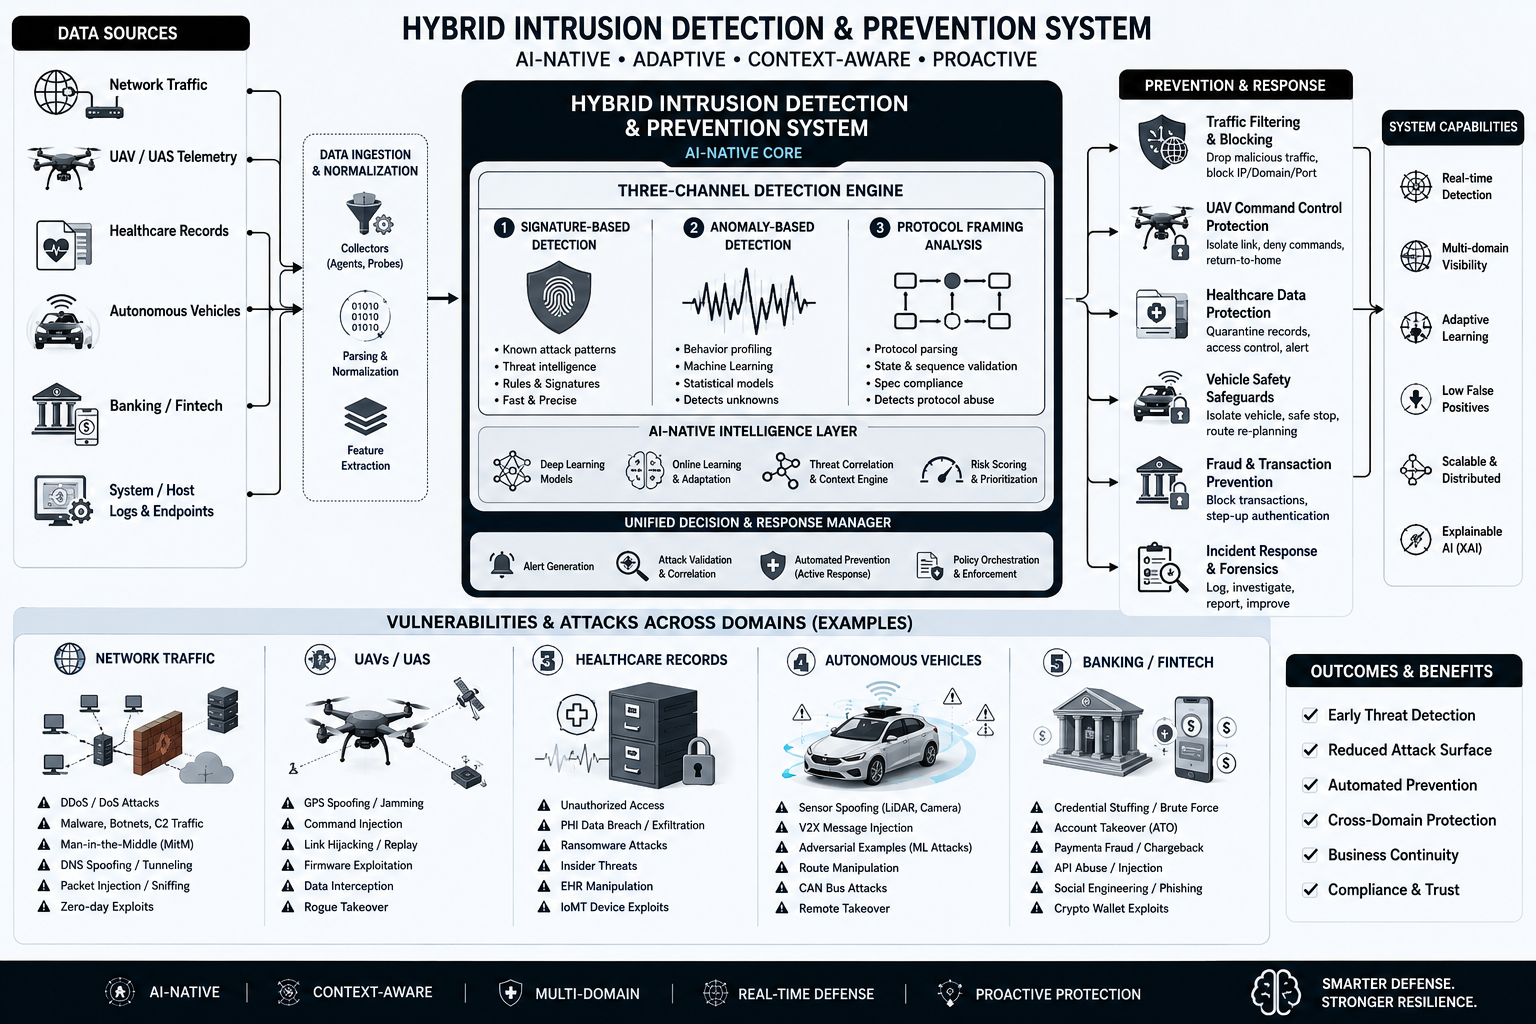
\includegraphics[width=\textwidth]{figures/fig_nidps_v1.png}
\caption{Integrated diagram of the Hybrid~IDPS system: an
AI-native, adaptive, context-aware, and proactive defensive
solution. \textbf{Left}~--- data sources (network traffic, UAV
telemetry, healthcare records, autonomous vehicles, banking/
fintech traffic, system/host logs); \textbf{centre}~--- the
system core with three-channel detection (signature-based,
anomaly-based, protocol framing analysis), the AI-native
intelligence layer (deep-learning models, online learning,
threat correlation, risk scoring) and the unified
decision-and-response manager; \textbf{right}~--- the prevention
and response block (traffic filtering, UAV command-link
protection, healthcare data protection, vehicle safety
safeguards, fraud and transaction prevention, incident response
and forensics) and the system capabilities (real-time detection,
multi-domain visibility, adaptive learning, low false-positive
rate, scalability, explainable AI). The bottom panel lists the
characteristic vulnerability classes in each of the five showcase
sectors.}
\label{fig:hybrid_idps_executive}
\end{figure}

%%=====================================================================\section{Hybrid IDPS as the Object of Research: Definition, Classification, and Application Domains}
\label{sec:hybrid_idps_object}%%=====================================================================

A \emph{Hybrid Intrusion Detection and Prevention System}
(Hybrid~IDPS) is in this dissertation defined as an \emph{AI/ML-native}
software-hardware defensive complex for information systems that
integrates the three canonical types of information-security
detection~--- \emph{signature-based} (deterministic matching against a
database of known attack patterns), \emph{anomaly-based} (statistical
or learned deviation from a normal behavioural profile), and
\emph{protocol-analysis-based} (context-aware analysis of the
correctness of network, application, and industrial protocols and
their states)~--- augmented by learnable models on each of the three
channels and supplemented with automatic response facilities and
interfaces to external event-logging and response systems (SIEM/SOAR). Unlike \emph{conventional} industry IDPS products (Snort, Suricata,
Zeek, Cisco~IPS, Palo Alto~Threat~Prevention), a Hybrid~IDPS in the
sense of this dissertation differs from classical IDS implementations
in \emph{four} systematic properties:
\emph{(i)}~\emph{hybridity} of detection~--- the verdict on the
presence of an intrusion is produced by the combination of multiple
independent detectors (signature, anomaly, protocol-analysis),
statistical features, and learned models with different degrees of
explainability;
\emph{(ii)}~\emph{adaptability} to the application domain~--- the
same base architecture can be instantiated for the protection of
network traffic, UAV systems, banking/fintech infrastructure,
medical data, industrial Internet-of-Things, and other domains by
changing the formal representation of input data;
\emph{(iii)}~\emph{closed-loop response}~--- in addition to detection,
a Hybrid~IDPS can initiate active countermeasures by modifying
firewall rules, isolating nodes, switching sensor pipelines, or
relaying events to a SOAR orchestrator;
\emph{(iv)}~\emph{AI-nativeness}~--- the learnable Models~M1--M7
developed in Chapter~\ref{ch:methods} are integrated across all three
detection channels (signature, anomaly, protocol-analysis) so as to
systematically overcome the three inefficiencies of conventional
IDPS noted in the Introduction: the 30--90-day signature-database
lag, the $10^{-2}$--$10^{-1}$ false-alert rate per normal flow, and
the quadratic cost of protocol analysis in the number of protocols
and states.

\subsection{Classification of Hybrid IDPS}
\label{subsec:idps_classification}

IDPS systems known in the literature admit classification along five
orthogonal axes: by the detection method employed, by the scope of
the observed environment, by the network topology of deployment, by
the character of response, and by the protocol-stack layer. The
structure of the classification is shown in
Fig.~\ref{fig:orga_classes_idps}.

\begin{figure}[htbp]
\centering
\resizebox{\textwidth}{!}{%
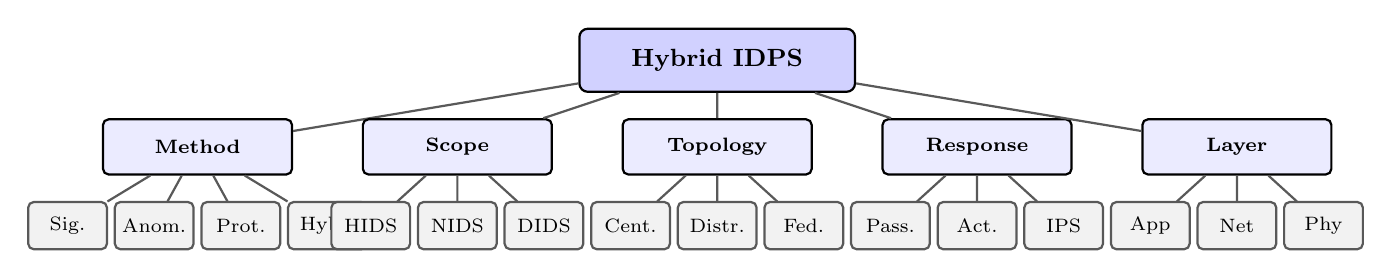
\begin{tikzpicture}[
  font=\footnotesize,
  level 1/.style={sibling distance=33mm, level distance=11mm},
  level 2/.style={sibling distance=11mm, level distance=10mm},
  root/.style={draw,rounded corners=3pt,fill=blue!18,
    minimum width=3.5cm,minimum height=8mm,align=center,
    font=\small\bfseries,thick},
  cat/.style={draw,rounded corners=2pt,fill=blue!8,
    minimum width=2.4cm,minimum height=7mm,align=center,
    font=\scriptsize\bfseries,thick},
  leaf/.style={draw,rounded corners=2pt,fill=gray!10,
    minimum width=1.0cm,minimum height=6mm,align=center,
    font=\scriptsize,inner sep=2pt},
  edge from parent/.style={draw,gray!70!black,thick}]
\node[root] {Hybrid IDPS}
  child {node[cat] {Method}
    child {node[leaf] {Sig.}}
    child {node[leaf] {Anom.}}
    child {node[leaf] {Prot.}}
    child {node[leaf] {Hybr.}}}
  child {node[cat] {Scope}
    child {node[leaf] {HIDS}}
    child {node[leaf] {NIDS}}
    child {node[leaf] {DIDS}}}
  child {node[cat] {Topology}
    child {node[leaf] {Cent.}}
    child {node[leaf] {Distr.}}
    child {node[leaf] {Fed.}}}
  child {node[cat] {Response}
    child {node[leaf] {Pass.}}
    child {node[leaf] {Act.}}
    child {node[leaf] {IPS}}}
  child {node[cat] {Layer}
    child {node[leaf] {App}}
    child {node[leaf] {Net}}
    child {node[leaf] {Phy}}};
\end{tikzpicture}%
}
\caption{Hierarchical classification of Hybrid IDPS along five
orthogonal axes. By detection method~--- signature-based
(deterministic lookup against a database of known patterns),
anomaly-based (statistical or learned deviation from a normal
profile), protocol-analysis-based (context-aware analysis of the
correctness of network, application, and industrial protocols and
their states), and hybrid (combination of the three preceding,
augmented with the learnable Models~M1--M7). By scope~---
host-based (HIDS), network-based (NIDS), and distributed (DIDS).
By deployment topology~--- centralised, distributed, federated.
By response character~--- passive (alerting only), active
(in-line intervention), and IPS (full blocking). By stack
layer~--- application, network, and physical.}
\label{fig:orga_classes_idps}
\end{figure}

This dissertation focuses primarily on hybrid systems with
distributed topology operating at the network and application layers
with active response.

\subsection{Application Domains of Hybrid IDPS}
\label{subsec:idps_sectors}

A Hybrid IDPS as a universal defensive contour is applicable across
a wide spectrum of domains. Figure~\ref{fig:orga_apps_idps}
systematises seven practically significant sectors, each of which is
treated below with brief problem-statement information on the attack
surface and the specifics of integrating defensive models.

\begin{figure}[htbp]
\centering
\resizebox{\textwidth}{!}{%
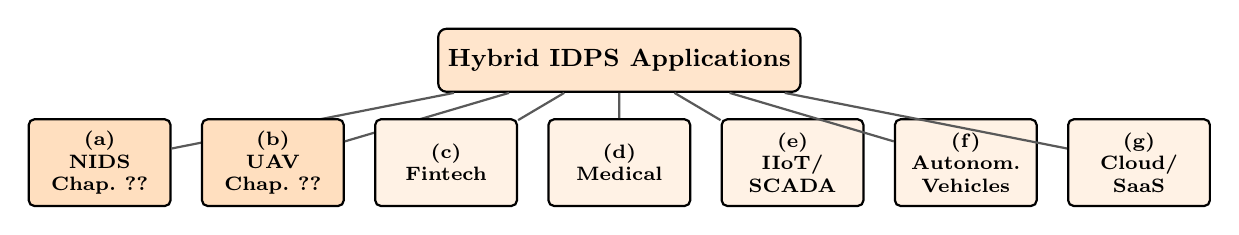
\begin{tikzpicture}[
  font=\footnotesize,
  level 1/.style={sibling distance=22mm, level distance=13mm},
  root/.style={draw,rounded corners=3pt,fill=orange!20,
    minimum width=4.6cm,minimum height=8mm,align=center,
    font=\small\bfseries,thick},
  sec/.style={draw,rounded corners=2pt,fill=orange!10,
    minimum width=1.8cm,minimum height=11mm,align=center,
    font=\scriptsize\bfseries,thick,inner sep=2pt},
  edge from parent/.style={draw,gray!70!black,thick}]
\node[root] {Hybrid IDPS Applications}
  child {node[sec,fill=orange!25] {(a)\\NIDS\\\scriptsize Chap.~\ref{ch:platform}}}
  child {node[sec,fill=orange!25] {(b)\\UAV\\\scriptsize Chap.~\ref{ch:uav}}}
  child {node[sec] {(c)\\Fintech}}
  child {node[sec] {(d)\\Medical}}
  child {node[sec] {(e)\\IIoT/\\SCADA}}
  child {node[sec] {(f)\\Autonom.\\Vehicles}}
  child {node[sec] {(g)\\Cloud/\\SaaS}};
\end{tikzpicture}%
}
\caption{Application domains of Hybrid IDPS. Sectors~(a) and~(b)
are treated in this work as showcase applications and are presented
in detail in Chapters~\ref{ch:platform} (network traffic analysis)
and~\ref{ch:uav} (UAV protection). Sectors~(c)--(g) are presented as
overview material with attack surface and defensive-model
integration mode for each.}
\label{fig:orga_apps_idps}
\end{figure}

Seven practically significant application sectors of Hybrid IDPS are systematised in Table~\ref{tab:idps_sectors}. Each sector is characterised by a specific attack surface and special requirements for integrating defensive models; key quantitative vulnerability indicators are retained in the attack-surface column with their respective citations.

\begin{table}[htbp]
\centering
\caption{Hybrid IDPS application domains: attack surface and special requirements.}
\label{tab:idps_sectors}
\small
\setlength{\tabcolsep}{4pt}
\begin{tabular}{p{2.8cm} p{6.5cm} p{5.0cm}}
\toprule
\textbf{Domain} & \textbf{Attack surface} & \textbf{Special requirements} \\
\midrule
(a)~Network traffic (NIDS) & Port scanning, service exploitation, DoS/DDoS, lateral movement, C2 channels, exfiltration, post-quantum protocol transitions; 46--83-dim vectors (CIC-IoT-2023, CSE-CICIDS-2018, UNSW-NB15) & Integration with signature engines (Snort, Suricata); SIEM alerts; see Chap.~\ref{ch:platform} \\
\addlinespace
(b)~UAV & GNSS spoofing/jamming, EW, adversarial attacks on onboard vision, autopilot policy poisoning, command-link hijacking, kinetic and biological threats & Graph representation of UAV operational environment; M1--M7 apparatus unchanged; see Chap.~\ref{ch:uav} \\
\addlinespace
(c)~Fintech & Carding, money laundering, raid-style transactional attacks (MonTi~\cite{MonTi2025}: CARE-GNN/PC-GNN/GAGA error from 25.7\% to 68.6\%), credential spoofing, phishing & Class imbalance ($<\!1\%$ fraud); Byzantine-resilient federated learning across banks \\
\addlinespace
(d)~Medical & Edge-sensitivity attacks on GIN (AUC drop to 25\% on MoleculeNet, toxic compounds as safe~\cite{EdgeSensitivity2025}), model inversion, membership inference, poisoning of clinical-trial graphs & $(\varepsilon,\delta)$-DP training; calibrated epistemic uncertainty \\
\addlinespace
(e)~IIoT/SCADA & PLC state manipulation, sensor signal replay, timestamp attacks; federated detector poisoning causes accuracy collapse from 94.2\% to 30.0\% under non-i.i.d.~\cite{FerragPoisoning2023} & Specialised protocols (\texttt{Modbus}, \texttt{DNP3}, \texttt{IEC~61850}, \texttt{OPC-UA}, \texttt{S7}); deterministic tens-of-ms latency \\
\addlinespace
(f)~Autonomous vehicles & Adversarial physical patches on traffic signs, GNSS spoofing, falsified V2X injection, trajectory-planner poisoning & Sensor-fusion graph (camera, LiDAR, radar, INS); calibrated uncertainty as safe-mode trigger \\
\addlinespace
(g)~Cloud/SaaS & Container escape, IAM abuse, supply-chain attacks, image substitution; PROVNINJA~\cite{PROVNINJA2023} reduces provenance-IDS detection to 59\% & East--west API traffic via service mesh (\texttt{Istio}, \texttt{Linkerd}); multi-tenant isolation \\
\bottomrule
\end{tabular}
\end{table}

Full system-level realisations for the two showcase sectors~--- (a)~network traffic protection and~(b)~UAV protection~--- are presented in Chapters~\ref{ch:platform} and~\ref{ch:uav}; sectors~(c)--(g) are realised on the basis of Models M1--M7 developed in Chapter~\ref{ch:methods}.

%% Anchor labels preserved for cross-references from other chapters:
\phantomsection\label{subsubsec:sector_nids}%
\phantomsection\label{subsubsec:sector_uav}%
\phantomsection\label{subsubsec:sector_fintech}%
\phantomsection\label{subsubsec:sector_medical}%
\phantomsection\label{subsubsec:sector_iiot}%
\phantomsection\label{subsubsec:sector_av}%
\phantomsection\label{subsubsec:sector_cloud}%

\iffalse
ORIGINAL TEXT (collapsed into Table~\ref{tab:idps_sectors}):

Network traffic protection is historically the first and most
extensively studied application area of IDPS. The object of
observation is a sequence of network packets and flows aggregated
into multidimensional feature vectors (46- to 83-dimensional vectors
in the CIC-IoT-2023, CSE-CICIDS-2018, and UNSW-NB15 benchmarks).

\paragraph{(b) Unmanned Aerial Vehicle Protection (UAV)}\label{subsubsec:sector_uav}

UAV protection is a showcase extension of Hybrid IDPS beyond the
traditional network perimeter. The object of observation is a
heterogeneous stream of onboard-sensor telemetry (INS/GNSS, LiDAR,
optical flow, engine and payload state) combined with the
command-and-telemetry channel onboard--droneport--cloud.

\paragraph{(c) Banking and Fintech Infrastructure Protection}\label{subsubsec:sector_fintech}

The protected object is the graph of transactions between accounts,
payment cards, points of sale, and fast-payment interfaces. The
attack surface includes carding, money laundering, raid-style
transactional attacks against fraud detectors (the
MonTi attack~\cite{MonTi2025} nearly triples the classification
error of CARE-GNN/PC-GNN/GAGA fraud detectors from 25.7\% to 68.6\%),
credential spoofing, phishing, and attacks against credit-scoring
systems.

\paragraph{(d) Protection of Medical Information Systems}\label{subsubsec:sector_medical}

The protected object is the graph of electronic medical records,
patient--clinician--laboratory interaction graphs, and molecular-
representation graphs in pharmacology tasks. The attack surface
includes edge-sensitivity attacks on graph-isomorphism networks
(AUC drops of up to 25\% on MoleculeNet benchmarks, with toxic
compounds classified as safe~\cite{EdgeSensitivity2025}), attacks on
the confidentiality of training data (model inversion, membership
inference), and poisoning of clinical-trial graphs.

\paragraph{(e) Industrial Internet-of-Things and ICS/SCADA Protection}\label{subsubsec:sector_iiot}

The industrial Internet-of-Things and industrial control systems
(ICS/SCADA) differ technically from traditional NIDS environments
in three respects that make IIoT/SCADA a separate application
sector of Hybrid IDPS rather than a special case of sector~(a):
\emph{(i)}~the protocol stack rests on specialised industrial
protocols (\texttt{Modbus}, \texttt{DNP3}, \texttt{IEC~61850},
\texttt{OPC-UA}, \texttt{S7}) with the semantics of control
registers, absent in the TCP/IP stack;
\emph{(ii)}~operational constraints require deterministic response
latency within tens of milliseconds, ruling out heavy inefficient
models;
\emph{(iii)}~the threat model includes industry-specific classes~---
manipulation of programmable-logic-controller (PLC) state, replay
of sensor signals, and attacks against time-synchronisation
timestamps. Poisoning of training data of federated intrusion
detectors in IIoT networks has been documented as the cause of an
accuracy collapse from 94.2\% to 30.0\% under non-i.i.d.\ training
conditions~\cite{FerragPoisoning2023}.

\paragraph{(f) Autonomous Vehicle Protection}\label{subsubsec:sector_av}

In autonomous vehicles the protected object is the sensor-fusion
graph (camera, LiDAR, radar, INS), the interaction graph with other
participants via V2X/V2I channels, and the software-component graph
of the autopilot. The attack surface includes physical adversarial
patches on traffic signs, GNSS spoofing, injection of falsified V2X
messages, and poisoning of the trajectory planner.

\paragraph{(g) Cloud and SaaS Infrastructure Protection}\label{subsubsec:sector_cloud}

Cloud and SaaS infrastructure protection also differs technically
from traditional NIDS environments and is not reducible to
sector~(a) for the following reasons:
\emph{(i)}~the primary observable stream is not the stream of
network packets but the stream of application-programming-interface
(API) calls between microservices (so-called east--west traffic),
observed via the service mesh infrastructure
(\texttt{Istio}, \texttt{Linkerd});
\emph{(ii)}~mandatory \emph{multi-tenant} isolation between cloud
tenants is required, absent in traditional network environments;
\emph{(iii)}~the threat model includes cloud-specific classes~---
container escape, abuse of identity-and-access-management (IAM)
credentials, supply-chain attacks against software, and container-
image substitution. The PROVNINJA attack~\cite{PROVNINJA2023}, which
reduces detection in provenance-based GNN systems to 59\%,
documents the necessity of protecting this sector.
\fi

%%=====================================================================
\section{Models and Algorithms Used in Hybrid IDPS: A Taxonomy}
\label{sec:idps_models_taxonomy}%%=====================================================================

The collection of models and algorithms used in Hybrid IDPS is
systematised in Fig.~\ref{fig:orga_models_idps} across five families:
statistical models, classical machine-learning algorithms, deep-
learning models, hybrid approaches, and game-theoretic algorithms. Graph neural networks (GNNs) are treated as one leaf of the deep-
learning branch~--- alongside convolutional, recurrent, transformer
models, and state-space models~--- rather than as the central
paradigm.

\begin{figure}[htbp]
\centering
\resizebox{\textwidth}{!}{%
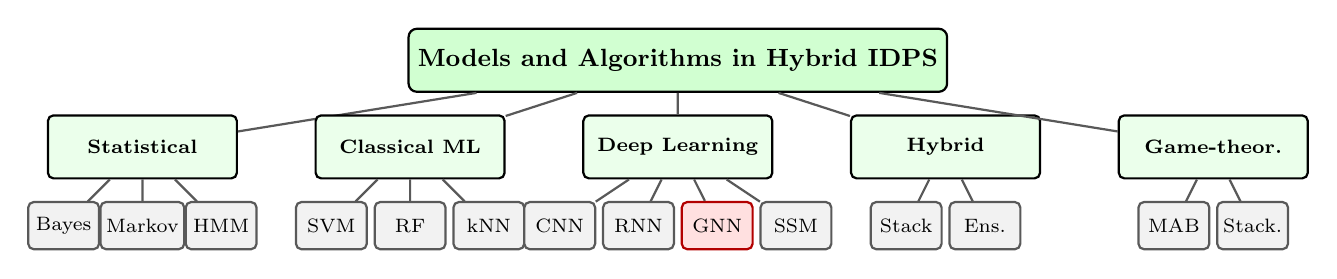
\begin{tikzpicture}[
  font=\footnotesize,
  level 1/.style={sibling distance=34mm, level distance=11mm},
  level 2/.style={sibling distance=10mm, level distance=10mm},
  root/.style={draw,rounded corners=3pt,fill=green!18,
    minimum width=4.2cm,minimum height=8mm,align=center,
    font=\small\bfseries,thick},
  fam/.style={draw,rounded corners=2pt,fill=green!8,
    minimum width=2.4cm,minimum height=8mm,align=center,
    font=\scriptsize\bfseries,thick},
  leaf/.style={draw,rounded corners=2pt,fill=gray!10,
    minimum width=0.9cm,minimum height=6mm,align=center,
    font=\scriptsize,inner sep=2pt},
  hi/.style={draw=red!70!black,fill=red!12,thick},
  edge from parent/.style={draw,gray!70!black,thick}]
\node[root] {Models and Algorithms in Hybrid IDPS}
  child {node[fam] {Statistical}
    child {node[leaf] {Bayes}}
    child {node[leaf] {Markov}}
    child {node[leaf] {HMM}}}
  child {node[fam] {Classical ML}
    child {node[leaf] {SVM}}
    child {node[leaf] {RF}}
    child {node[leaf] {kNN}}}
  child {node[fam] {Deep Learning}
    child {node[leaf] {CNN}}
    child {node[leaf] {RNN}}
    child {node[leaf,hi] {GNN}}
    child {node[leaf] {SSM}}}
  child {node[fam] {Hybrid}
    child {node[leaf] {Stack}}
    child {node[leaf] {Ens.}}}
  child {node[fam] {Game-theor.}
    child {node[leaf] {MAB}}
    child {node[leaf] {Stack.}}};
\end{tikzpicture}%
}
\caption{Taxonomy of models and algorithms used in Hybrid IDPS.
Graph neural networks (highlighted in red) are one leaf of the
deep-learning branch alongside convolutional networks (CNN),
recurrent networks (RNN), state-space models (SSM) and stochastic
differential equations (SDE), and not the central paradigm. The
Models M1--M7 developed in Chapter~\ref{ch:methods} borrow
constructs from several branches simultaneously
(see Table~\ref{tab:models_to_methods}).}
\label{fig:orga_models_idps}
\end{figure}

Each family of models has characteristic strengths and weaknesses
that determine its area of applicability in Hybrid IDPS tasks. Statistical models and classical machine-learning algorithms are
efficient on low-dimensional tabular features and provide
interpretable decision boundaries, but they cannot automatically
extract abstract representations from raw sensor streams and do
not scale to million-node graphs.

%%---------------------------------------------------------------------
\subsection{Modern Commercial AI-Augmented IDPS Products}
\label{subsec:commercial_ai_idps}

%%---------------------------------------------------------------------

Since 2023--2025, leading information-security vendors have introduced a class of \emph{AI-augmented} commercial detection and response platforms layered above classical signature-based and behavioural engines. A systematic review of seven representative products in Table~\ref{tab:ai_idps_products} positions the RobustIDPS.ai framework developed in this work against the prevailing industrial state of the art.

\iffalse
\begin{enumerate}[leftmargin=2em, itemsep=0pt]

\item \textbf{CrowdStrike Falcon with the Charlotte~AI module}~---
an EDR/XDR platform with an embedded LLM assistant for accelerated
alert triage and automated generation of response playbooks; the
detection core relies on behavioural indicators of attack (IoA)
and process graphs. The declared advantage is reduction of SOC
analyst response time; the limitations are a closed rule corpus,
the absence of formal robustness certificates against adversarial
influence, and dependence on the CrowdStrike cloud back-end.

\item \textbf{SentinelOne Singularity with Purple~AI}~--- an
autonomous XDR platform with an agentic AI for natural-language
incident investigation; implements behavioural detection at the
endpoint level and automated rollback under ransomware. Limitations
relevant to the present work: absence of a formal privacy model
for federated training on data from multiple customers, and the
absence of certified resilience against poisoning of training data.

\item \textbf{Microsoft Security Copilot}~--- a layer on top of
the Defender~XDR / Sentinel SIEM family powered by GPT-family
LLMs; oriented toward augmenting the SOC operator (incident
summarisation, KQL query generation, response-plan construction).
The principal limitation is that the LLM decisions are not
accompanied by quantitative uncertainty estimates and carry no
formal robustness guarantees under adversarial prompts
(prompt-injection).

\item \textbf{Google Cloud Threat Intelligence (Mandiant +
Gemini)}~--- integrates Mandiant indicators of compromise with the
Gemini LLM assistant for attribution and threat prioritisation;
the strong side is aggregated threat-intelligence feeds, the weak
side is the closed-model nature and the absence of guarantees for
on-premises deployments.

\item \textbf{Cisco AI Endpoint Analytics / Hypershield}~---
targets network segmentation and workstation-level anomaly
detection by means of learnable device-identification models;
constitutes a commercial counterpart of the feature-learning
models for NIDPS reviewed in Section~1.6.

\item \textbf{IBM QRadar SIEM AI Assistant} and \textbf{Palo~Alto
Networks Cortex~XSIAM}~--- AI-augmented SIEM/SOAR platforms;
they provide automated event correlation and analyst
recommendation systems but neither supply certified guarantees
of adversarial resilience nor implement federated learning across
organisations.

\end{enumerate}
\fi
\begin{table}[htbp]
\centering
\caption{AI-augmented commercial IDPS products (2023--2025): approach and key limitations.}
\label{tab:ai_idps_products}
\small
\setlength{\tabcolsep}{4pt}
\begin{tabular}{p{2.7cm} p{2.0cm} p{4.5cm} p{4.8cm}}
\toprule
\textbf{Product} & \textbf{Vendor} & \textbf{Approach} & \textbf{Key limitations} \\
\midrule
Falcon + Charlotte~AI & CrowdStrike & EDR/XDR with LLM assistant; behavioural IoA and process graphs & Closed rule corpus; no formal robustness certificates; cloud back-end dependence \\
\addlinespace
Singularity + Purple~AI & SentinelOne & Autonomous XDR with agentic AI for natural-language incident investigation; ransomware rollback & No formal privacy model for federated training; no certified resilience to poisoning \\
\addlinespace
Security Copilot & Microsoft & Layer over Defender~XDR/Sentinel SIEM on GPT-family LLMs; incident summarisation, KQL generation & No quantitative uncertainty estimates; no guarantees against prompt-injection \\
\addlinespace
Mandiant + Gemini & Google Cloud & Integration of Mandiant IoCs with Gemini LLM for attribution and prioritisation & Closed-model nature; no guarantees for on-premises deployments \\
\addlinespace
AI Endpoint Analytics / Hypershield & Cisco & Network segmentation and workstation-level anomaly detection via learnable device identification & Commercial counterpart of NIDPS feature-learning models; no robustness certificates \\
\addlinespace
QRadar SIEM AI Assistant & IBM & AI-augmented SIEM/SOAR: automated event correlation and analyst recommendations & No certified adversarial guarantees; no cross-organisation federated learning \\
\addlinespace
Cortex~XSIAM & Palo~Alto Networks & AI-augmented SIEM/SOAR: extended analytics and response automation & No certified adversarial guarantees; no cross-organisation federated learning \\
\bottomrule
\end{tabular}
\end{table}

\noindent A systematic analysis of the products listed above
shows that \emph{all} of them are pipeline overlays of LLM/EDR
on top of classical engines, in which the following are absent:
(i)~a unified mathematical model of Hybrid~IDPS as an object of
study with formal robustness guarantees, (ii)~certified resilience
against adversarial attacks with proofs by Lipschitz continuity or
randomised smoothing, (iii)~private distributed-training
algorithms with differential privacy and Byzantine-resilient
aggregation, (iv)~calibrated decomposition of epistemic and
aleatoric uncertainty. These four aspects constitute the
substantive distinction of the Models M1--M7 and the RobustIDPS.ai
platform developed in the present work from the commercial
AI-augmented IDPS products reviewed above; the quantitative
comparison is carried out in Chapter~\ref{ch:platform} (the
section ``Comparison with commercial and open-source
platforms'').

%%=====================================================================\section{Methods of Data Representation and Analysis in Intrusion Detection Systems}
\label{sec:data_representation_methods}

Four main families of data-representation and analysis methods are used in
modern intrusion-detection systems, each with its own effective range and
fundamental limitations.

\subsection{Signature-based Methods}

Signature-based methods (Snort, Suricata, Zeek) match network traffic against
a database of known attack patterns. They provide high precision on known
threats with low false-positive rates, but they fundamentally cannot detect
previously unknown (zero-day) attacks and lag the emergence of new threats
by 30--90~days~\cite{Roesch1999,Paxson1999}.

\subsection{Statistical Methods}

Statistical methods (HMM, GMM, OSSEC) model the normal distribution of
traffic features and detect deviations. They can detect new attack types
but scale poorly on high-dimensional flows and generate many false alarms
under changing environmental statistics.

\subsection{Machine-learning Methods}

Classical machine-learning methods (SVM, Random Forest, kNN) provide a
trade-off between interpretability and detection accuracy, but require
manual feature selection and do not automatically extract abstract
representations from raw data streams~\cite{Buczak2016}.

\subsection{Deep-learning Methods}

Deep-learning methods (convolutional, recurrent, graph neural networks,
transformers, state-space models) automatically extract features and
achieve the highest detection accuracy, but they suffer from adversarial
instability and high computational cost in real-time
operation~\cite{Ahmad2021,Ferrag2020}.

%%===================================================================\section{Problems and Vulnerabilities of Modern Intrusion Detection Models under Adversarial, Distributed, and Non-stationary Conditions}
\label{sec:idps_problems}%%=====================================================================

The set of problems considered in the work as motivating the
development of Models and algorithms M1--M7 is systematised in
Fig.~\ref{fig:orga_problems_idps}. The problems are distributed
across five cross-cutting axes: robustness against adversarial
influence, accuracy under non-stationarity and class imbalance,
inference efficiency under limited budgets, differential privacy in
distributed environments, and non-stationary adaptation under
distribution shift.

\begin{figure}[htbp]
\centering
\resizebox{\textwidth}{!}{%
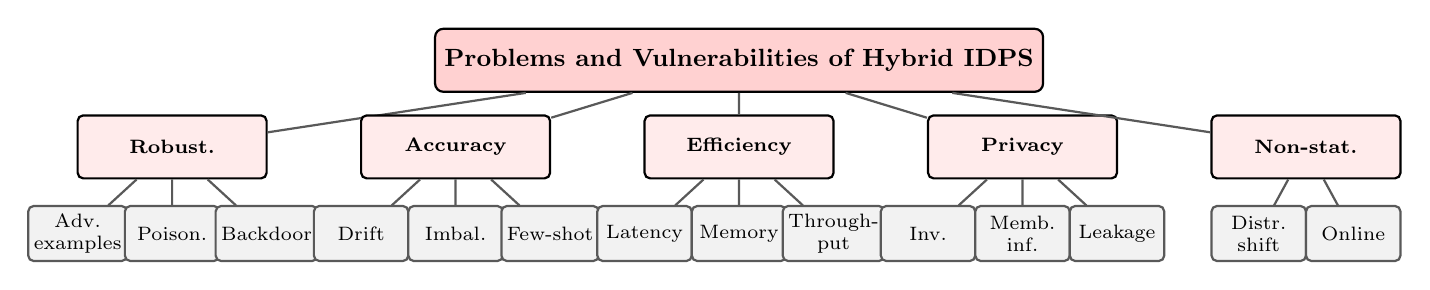
\begin{tikzpicture}[
  font=\footnotesize,
  level 1/.style={sibling distance=36mm, level distance=11mm},
  level 2/.style={sibling distance=12mm, level distance=11mm},
  root/.style={draw,rounded corners=3pt,fill=red!18,
    minimum width=4.6cm,minimum height=8mm,align=center,
    font=\small\bfseries,thick},
  ax/.style={draw,rounded corners=2pt,fill=red!8,
    minimum width=2.4cm,minimum height=8mm,align=center,
    font=\scriptsize\bfseries,thick},
  leaf/.style={draw,rounded corners=2pt,fill=gray!10,
    minimum width=1.2cm,minimum height=7mm,align=center,
    font=\scriptsize,inner sep=2pt},
  edge from parent/.style={draw,gray!70!black,thick}]
\node[root] {Problems and Vulnerabilities of Hybrid IDPS}
  child {node[ax] {Robust.}
    child {node[leaf] {Adv.\\examples}}
    child {node[leaf] {Poison.}}
    child {node[leaf] {Backdoor}}}
  child {node[ax] {Accuracy}
    child {node[leaf] {Drift}}
    child {node[leaf] {Imbal.}}
    child {node[leaf] {Few-shot}}}
  child {node[ax] {Efficiency}
    child {node[leaf] {Latency}}
    child {node[leaf] {Memory}}
    child {node[leaf] {Through-\\put}}}
  child {node[ax] {Privacy}
    child {node[leaf] {Inv.}}
    child {node[leaf] {Memb.\\inf.}}
    child {node[leaf] {Leakage}}}
  child {node[ax] {Non-stat.}
    child {node[leaf] {Distr.\\shift}}
    child {node[leaf] {Online}}};
\end{tikzpicture}%
}
\caption{Systematisation of problems and vulnerabilities motivating
the development of Models M1--M7. Each of the five axes is covered
by one or several developed models (direct mapping is given in
Table~\ref{tab:models_to_methods} after the analysis of existing
limitations).}
\label{fig:orga_problems_idps}
\end{figure}

The correspondence between the axes of
Fig.~\ref{fig:orga_problems_idps} and the developed models gives a
direct mapping of the research directions of the specialty 2.3.1
passport (items~4 and~5) onto the contributions of the dissertation:
the \emph{robustness} axis is covered by Models~M1, M4, and~M5--M6;
the \emph{accuracy} axis~--- by~M1, M3, and~M5--M6;
the \emph{efficiency} axis~--- by~M4 and~M7;
the \emph{privacy} axis~--- by~M2;
the \emph{non-stationarity} axis~--- by~M1, M3, and~M6.

%%=====================================================================\section{Graph-based Representation of Network Traffic as the Basis for Analysing Complex Network Interactions}
\label{sec:graph_representation}

Classical intrusion-detection models operate on individual packets or
flows in isolation, whereas real attacks develop within the \emph{structure}
of network interactions among hosts, services, and users. Graph-based
representation enables the systematic encoding of these relationships and
the application of graph-analytical algorithms to them.

%%===================================================================\section{Graph Neural Networks for Network Traffic Analysis}
\label{sec:gnn_vulnerability}%%=====================================================================

\subsection{Message-Passing Architecture and Neighbourhood Aggregation}

Graph neural networks~\cite{Kipf2017,Velickovic2018,Hamilton2017} extend deep learning to non-Euclidean relational data by iteratively aggregating information from a node's neighbours. The canonical message-passing formulation updates the representation of node $v$ at layer $k+1$ as.

\begin{equation}
\bh_v^{(k+1)}
= \phi\!\Bigl(\bh_v^{(k)},\;
  \bigoplus_{u\in\calN(v)}
    \psi\!\bigl(\bh_u^{(k)},\, \mathbf{e}_{uv}\bigr)\Bigr),
\label{eq:ch1_mp}
\end{equation}where $\phi$ and $\psi$ are learnable functions, $\bigoplus$ is a permutation-invariant aggregator (sum, mean, or max), and $\calN(v)$ denotes the neighbourhood of $v$. This framework encompasses GCN~\cite{Kipf2017}, GAT~\cite{Velickovic2018}, GraphSAGE~\cite{Hamilton2017}, and their temporal extensions~\cite{Xu2020tgat,Rossi2020,Pei2020tgn,Kazemi2020,Schlichtkrull2018}.

Graph neural networks are deployed in healthcare (molecular property prediction on atom-bond graphs, patient-interaction graphs for treatment recommendations), finance (transaction-graph analysis for fraud detection and anti-money laundering), cybersecurity (network-traffic graphs for intrusion detection), industrial systems (sensor-fusion graphs for SCADA and ICS monitoring), and autonomous systems (sensor-fusion graphs for perception)~\cite{Goodfellow2014gan,Gilmer2017,Gilmer2018,Ying2021,Wu2021,Luo2021}. The breadth of these deployments underscores the urgency of robustness analysis.

\subsection{The Dual-Input Vulnerability}

Unlike conventional neural networks that receive a single data tensor, a graph neural network receives two inputs simultaneously: numerical \emph{input data} $\mathbf{X}\in\mathbb{R}^{n\times d}$ (the feature matrix encoding entity attributes) and relational \emph{input structure} $\mathbf{A}\in\{0,1\}^{n\times n}$ (the adjacency matrix encoding pairwise connectivity). The network produces its output by propagating data along the structure through iterative neighbourhood aggregation, and perturbation of \emph{either} input --- the data or the structure --- can compromise the output~\cite{Zuegner2018,Bojchevski2019,Dai2018}.

\subsection{Documented Failures in Safety-Critical Domains}

The vulnerability of graph neural networks is not a theoretical concern --- it has been documented in peer-reviewed studies across four safety-critical domains. In healthcare, edge-sensitivity gradient attacks on Graph Isomorphism Networks caused approximately 25\% AUC degradation on MoleculeNet benchmarks (Tox21, ClinTox, SIDER), with toxic compounds misclassified as safe~\cite{EdgeSensitivity2025}.

%%=====================================================================\section{Continuous-Time Dynamics on Evolving Graphs}
\label{sec:ct_dynamics}%%=====================================================================

\subsection{Neural Ordinary Differential Equations for Graph Representation}

Chen et al.~\cite{Chen2018} introduced neural ordinary differential equations (neural ODEs), replacing the discrete layer-by-layer updates of conventional networks with a continuous-depth parameterisation:.

\begin{equation}
\frac{d\bh(t)}{dt} = f_\theta\!\bigl(\bh(t),\, t\bigr),
\label{eq:ch1_ode}
\end{equation}where $f_\theta$ is a neural network parameterising the vector field. The output at any time $T$ is obtained by numerically integrating Equation~\eqref{eq:ch1_ode} from $t=0$ to $t=T$ using adaptive-step solvers, and gradients are computed memory-efficiently through the adjoint sensitivity method~\cite{Pontryagin1962}.

Temporal graph networks such as TGAT~\cite{Xu2020tgat} and TGN~\cite{Rossi2020} model time-stamped interactions on evolving graphs, but they operate in discrete time --- each event triggers a single update step. This forces irregular graph events onto a fixed computational clock, losing information about the precise timing and ordering of interactions between steps.

\subsection{Lipschitz Stability and the Gr\"{o}nwall Bound}

The key advantage of continuous-time formulations is their inherent smoothness. Because representations evolve according to a differential equation with a bounded Lipschitz constant $L_g$, the Gr\"{o}nwall inequality provides a closed-form robustness certificate:.

\begin{equation}
\|\mathbf{h}_1(T) - \mathbf{h}_2(T)\| \leq e^{L_g T}\|\mathbf{x}_1 - \mathbf{x}_2\|,
\label{eq:ch1_gronwall}
\end{equation}where $\mathbf{h}_i(T)$ is the hidden state of trajectory $i$ at time $T$ and $\mathbf{x}_i$ is the initial input. This bound states that small perturbations of the input can only cause bounded, smooth changes in the output --- the smoothness of the governing flow mathematically limits how much an adversary can move the prediction.

Randomised smoothing~\cite{Cohen2019} and interval bound propagation~\cite{Gowal2019} provide alternative certification pathways, but they were designed for image classifiers and do not account for the combinatorial structure of graph adjacency matrices or the continuous-time integration of neural ODEs. Lecuyer et al.~\cite{Lecuyer2019} connected differential privacy to certified robustness, and Salman et al.~\cite{Salman2019} combined randomised smoothing with adversarial training.

\subsection{Limitations of Existing Continuous-Time Approaches}

Despite the theoretical promise, no existing work derives certified robustness bounds from the smoothness of the governing differential equation on temporally evolving graph topologies. Existing continuous-time graph models either operate on static graphs~\cite{Chamberlain2021} or handle temporal edges without Lipschitz analysis~\cite{Xu2020tgat,Rossi2020,Pei2020tgn,Kazemi2020,Wang2021tedic}.

\noindent\textbf{Gap~1:} \emph{No certified robustness under continuous-time graph dynamics.} No existing architecture provides formally certified robustness bounds for graph neural networks operating in continuous time on temporally evolving topologies, combining Lipschitz analysis of the governing vector field with memory-efficient adjoint training and multi-scale temporal dynamics.

\medskip
\noindent\textit{Section summary.} Continuous-time formulations offer a principled pathway to certified robustness through Lipschitz-bounded dynamics, but existing approaches do not extend to evolving graphs with temporal event streams. The next section examines how these models must be adapted for distributed environments where data cannot be centralised.

%%=====================================================================\section{Distributed Learning of Graph Models under Confidentiality Constraints}
\label{sec:distributed}%%=====================================================================

\subsection{Federated Learning Fundamentals}

McMahan et al.~\cite{McMahan2017} introduced Federated Averaging (FedAvg), enabling distributed training across multiple participants without centralising raw data. Each participant computes local gradient updates on its data fragment, and a central server aggregates these updates into a global model.

\subsection{Byzantine-Resilient Aggregation}

Standard federated averaging is vulnerable to Byzantine participants who submit corrupted gradient updates. Blanchard et al.~\cite{Blanchard2017} proposed Krum, which selects the update closest to its neighbours, while Yin et al.~\cite{Yin2018} showed that coordinate-wise trimmed means achieve minimax-optimal rates under Byzantine corruption.

\subsection{Differential Privacy and Optimal Transport}

Differential privacy~\cite{Dwork2006} formalises data-record-level confidentiality through the condition.

\begin{equation}
\Prob\bigl[\calM(\calD)\in S\bigr]
\;\le\;
e^{\epsilon}\;\Prob\bigl[\calM(\calD')\in S\bigr] + \delta,
\end{equation}and the moments-accountant composition~\cite{Abadi2016} enables precise tracking of the cumulative privacy expenditure across training rounds. Optimal transport~\cite{Villani2009,Cuturi2013} provides a geometry on probability distributions through the Wasserstein distance, offering a principled mechanism for aligning heterogeneous graph-fragment distributions across participants.

\medskip
\noindent\textbf{Gap~2:} \emph{Unfavourable privacy-utility trade-off in federated graphs.} No existing federated learning algorithm jointly provides Byzantine-resilient aggregation, formal $(\epsilon,\delta)$-differential privacy, and Wasserstein optimal-transport distributional alignment for graph-structured data, where the topology itself can be partially controlled by an adversary.

\medskip
\noindent\textit{Section summary.} Distributed graph learning requires simultaneous corruption tolerance, privacy protection, and distributional alignment --- a combination no existing method achieves. The next section examines the computational efficiency challenges that any deployed solution must overcome.

%%=====================================================================\section{Methods for Improving Computational Efficiency of Large-Scale Temporal Graph Processing}
\label{sec:efficiency}%%=====================================================================

\subsection{Quadratic Bottleneck of Graph Transformers}

Graph-transformer architectures~\cite{Vaswani2017,Ying2021} achieve strong results on graph-level tasks by allowing every node to attend to every other node. However, this self-attention mechanism scales quadratically ($\mathcal{O}(L^2)$) with the number of nodes or events, making it prohibitively expensive for large-scale temporal graphs with millions of interactions.

\subsection{Structured State-Space Models}

Gu et al.~\cite{Gu2022} introduced structured state-space models (S4) that reformulate sequential processing as a linear dynamical system whose convolutional kernel is evaluated in $\mathcal{O}(L\log L)$ time through the Fast Fourier Transform. The selective variant (Mamba)~\cite{Dao2024} adds input-dependent gating for improved modelling of discrete tokens.

\subsection{Multi-Level Representations}

Temporal graphs in which nodes and edges carry different semantic types and evolve at different time scales require representations that capture structure at multiple levels of detail. Existing temporal GNNs learn a single, uniform embedding per node, which cannot resolve service-level patterns, trace-level dependencies, and node-level dynamics simultaneously.

\noindent\textbf{Gap~3:} \emph{Limited cross-distribution generalisation on temporal graphs.} No existing architecture learns multi-level temporal graph representations (service, trace, node) while simultaneously preventing catastrophic forgetting as the topology evolves and achieving computational savings through structured sparsity.

\medskip
\noindent\textbf{Gap~4:} \emph{Discrete-time constraints and quadratic cost.} Structured state-space models offering near-linear cost have not been adapted to graph data with formal robustness guarantees, progressive adversarial distillation, or PAC-Bayesian generalisation certificates.

\medskip
\noindent\textit{Section summary.} Efficiency and multi-level representation pose interrelated challenges: richer representations demand more computation, and efficient architectures lack robustness guarantees. The next section examines how deployed models must adapt to non-stationary conditions.

%%=====================================================================\section{Non-Stationary Adaptation and Uncertainty Quantification}
\label{sec:nonstationarity}%%=====================================================================

\subsection{Distribution Drift in Deployed Models}

Real graph data drifts after deployment: topologies evolve, attack patterns change, new protocols emerge, and static models silently lose accuracy without warning. This is unacceptable in safety-critical systems where a stale model is a dangerous model.

\subsection{Bayesian Approaches to Uncertainty}

Bayesian neural networks produce posterior predictive distributions that decompose total uncertainty into epistemic (model) and aleatoric (data) components~\cite{Gal2016,Blundell2015,Lakshminarayanan2017,Kendall2017}. Variational inference approximates the intractable posterior through parameterised distributions, enabling uncertainty estimation at the cost of additional forward passes (Monte Carlo dropout) or ensemble training.

\subsection{Online Learning with Sub-Linear Regret}

Online convex optimisation provides a framework for sequential decision-making under adversarial data streams, with algorithms such as follow-the-regularised-leader achieving sub-linear regret bounds~\cite{Shalev2012,Arjovsky2017}. The multiplicative weights update achieves $R(T)\leq\sqrt{T\log|S|}$ regret against the best fixed strategy in hindsight.

\noindent\textbf{Gap~5:} \emph{Forward incompatibility with protocol regime change.} No existing domain-specific foundation model combines ODE-augmented state-space processing with multi-task graph event sequence modelling for forward-compatible detection under evolving protocols. The post-quantum cryptographic landscape, from Shor's algorithm~\cite{Shor1997} through lattice-based constructions~\cite{Ducas2018,Proos2003} and code-based schemes~\cite{McEliece1978}, introduces fundamental changes to the statistical features observed on graph edges. The foundation model paradigm established by Brown et al.~\cite{Brown2020} and Devlin et al.~\cite{Devlin2019} has been extended to domain-specific applications, with Touvron et al.~\cite{Touvron2023} demonstrating open-weight alternatives and Wei et al.~\cite{Wei2022cot} establishing chain-of-thought reasoning capabilities that enable structured threat analysis.

\medskip
\noindent\textbf{Gap~6:} \emph{Unintegrated uncertainty and adversarial robustness.} No existing architecture combines variational Bayesian attention with hierarchical Gaussian process uncertainty quantification for graph-structured data, providing simultaneous epistemic--aleatoric decomposition, online drift detection, and sub-linear regret guarantees under adversarial non-stationarity.

\medskip
\noindent\textit{Section summary.} Non-stationary adaptation requires online learning with formal regret guarantees and calibrated uncertainty decomposition --- capabilities not available in existing graph architectures. The final gap concerns how these diverse guarantees can be unified into a single certification framework.

%%=====================================================================\section{Methods for Ensuring and Certifying Robustness of Machine-Learning Models}
\label{sec:certification}%%=====================================================================

\subsection{Game-Theoretic Threat Models}

Tambe~\cite{Tambe2011} and Sinha et al.~\cite{Sinha2018} formalised security resource allocation as Stackelberg games, where a defender commits to a strategy anticipating the adversary's best response. In the graph neural network context, the defender is the classifier and the adversary perturbs the graph to maximise misclassification.

\subsection{Existing Certification Methods}

Randomised smoothing~\cite{Cohen2019,Salman2019} provides probabilistic robustness certificates for continuous input spaces. Interval bound propagation~\cite{Gowal2019,Wong2018} provides deterministic bounds by propagating interval-valued inputs through the network.

\noindent\textbf{Gap~7:} \emph{Oversimplified game-theoretic threat models.} No existing unified certification framework combines game-theoretic strategy selection (Stackelberg equilibria with no-regret online learning), interval bound propagation, Lipschitz estimation on graph operators, and randomised smoothing adapted to discrete graph structures within a single methodology that couples all component methods through consistency regularisation.

\medskip
\noindent\textit{Section summary.} Existing certification methods address individual perturbation types in isolation and do not extend to the combinatorial structure of graphs or the compositional architecture of multi-method defence systems. A unified framework is needed to tie together all guarantees developed across the preceding sections.

%%=====================================================================
\section{Adversarial Machine Learning in Adjacent Safety-Critical Domains: the Case of Neural-Network UAV Navigation}
\label{sec:ch1_uav_related}

The principal target domain of the present dissertation~--- hybrid
network intrusion detection and prevention systems~--- is only
\emph{one} of the applications of the domain-independent methods
\textsf{M1}--\textsf{M7} formulated in Chapter~2. To confirm
domain-independence, Chapter~6 carries the framework over to the
neural-network navigation subsystem of unmanned aerial vehicles
(UAVs) operating under electronic-warfare (EW) and
adversarial-machine-learning pressure.

\subsection{Degradation of UAV Neural-Network Components under EW
Pressure}

Open military reviews and analytical briefs document an accelerating
degradation of UAV neural-network components as EW pressure grows. According to investigative journalism~\cite{wapo_excalibur_2024},
the hit rate of the GPS-guided M982~Excalibur artillery shell fell
from above~50\,\% to below~10\,\% within months in zones covered by
Russian EW assets.

\subsection{Adversarial Attacks on Aerial Visual Detectors}

Lian et~al.~\cite{lian_2022_uav} have shown that adaptive
adversarial patches against the aerial detectors YOLOv2--v5,
Faster~R-CNN and SSD on the VisDrone benchmark reduce mean average
precision (mAP) by 87.86~p.p.\ in the white-box and 85.48~p.p.\ in
the black-box regime. Du et~al.~\cite{du_2022_uav} obtained an
mAP drop of YOLOv3 from $\approx$0.95 to~$<$0.20 with physically
printed patches.

\subsection{Adversarial Attacks on Deep Reinforcement Learning
Policies}

Hickling, Aouf and Spencer~\cite{hickling_2023_uav} have shown that
the iterative BIM method drops the obstacle-course completion rate
of an APF+DDPG-PER UAV pilot from 97\,\% to 35\,\%, and proposed a
SHAP detector of adversarial influences with 80--91\,\% detection
rate. A review of adversarial attacks on UAV neural-network
components and existing defence methods has been presented in the
work of A.\,E.\,Lisin and S.\,G.\,Cherny~\cite{Lisin2023uav}.

\subsection{GNSS Spoofing and Drift-Evasive Attacks}

Borhani-Darian et~al.~\cite{borhani_2024_uav} have built a deep
convolutional network that detects spoofing at the signal level
through cross-ambiguity-function (CAF) features. Aigner
et~al.~\cite{aigner_2025_uav} have obtained a detection error of
0.16\,\% on the TEXBAT benchmark with a Seq2Seq Transformer
architecture.

\subsection{Graph Neural Networks in UAV-Swarm Tasks}

Mou et~al.~\cite{mou_2021_uav} have applied a GCN to self-healing
UAV-swarm communications. The hierarchical federated GAT
\cite{hfgat_2025_uav} delivers below-2\,\% collision rate at 500~UAVs
and Byzantine fraction $f<n/3$.

\subsection{Regulatory Context for UAVs}

In the Russian Federation, Government Decree No.~1701 of
30~November~2024~\cite{decree_1701} requires that UAVs above 250\,g
be equipped with certified communication, remote-identification and
cryptographic-information-protection means. \mbox{GOST~R~72118-2025}~\cite{GOST_R_72118_2025} regulates the
formalisation of AI threat models, and
\mbox{GOST~R~55679-2021}~\cite{GOST_R_55679_2021} sets general
requirements for unmanned aerial systems.

%%=====================================================================\section{Summary of Identified Research Gaps}
\label{sec:gap_summary}%%=====================================================================

The systematic analysis conducted in Sections~\ref{sec:gnn_vulnerability}--\ref{sec:certification} identifies seven research gaps that collectively define the open problem space addressed by this dissertation. Table~\ref{tab:gaps} maps each gap to the operating conditions and requirements it involves, and identifies the model/algorithm developed in Chapter~\ref{ch:methods} to address it.

\begin{table}[H]
\centering
\caption{Mapping of Hybrid IDPS problem axes identified in \S\ref{sec:idps_problems} to the Models and Algorithms M1--M7 developed in Chapter~\ref{ch:methods} (alignment with item~4 of the specialty 2.3.1 passport).}
\label{tab:models_to_methods}
\small
\setlength{\tabcolsep}{4pt}
\renewcommand{\arraystretch}{0.92}\begin{tabular}{p{3.0cm} p{4.5cm} p{6.5cm}}
\toprule
\textbf{Problem axis} & \textbf{Specific vulnerability} & \textbf{Developed Model / algorithm} \\
\midrule
Robustness     & Adversarial examples, poisoning, backdoors
               & M1 (CT-TGNN, Lipschitz certificate), M4 (MambaShield, PAC-Bayes), M5--M6 (stoch.\ transformer + UC-HGP), M7 (game-theoretic certification) \\
\addlinespace
Accuracy       & Concept drift, class imbalance, few-shot
               & M1 (multi-scale time constants), M3 (TripleE-TGNN multi-level representations), M5--M6 (calibrated uncertainty) \\
\addlinespace
Efficiency     & Inference latency, memory, throughput
               & M4 (MambaShield, $O(L\log L)$), M7 (uncertainty-guided strategy selection) \\
\addlinespace
Privacy        & Model inversion, membership inference, leakage
               & M2 (FedLLM-API, $(\varepsilon,\delta)$-DP + Byzantine resilience) \\
\addlinespace
Non-stationarity & Distribution shift, online learning
                 & M1 (CT-TGNN), M3 (elastic weight consolidation), M6 (UC-HGP Bayesian updates) \\
\bottomrule
\end{tabular}\end{table}

\begin{table}[htbp]\centering\small
\caption{Seven identified research gaps, their condition--requirement coverage, and the methods proposed to address them in this dissertation.}
\label{tab:gaps}
\small
\renewcommand{\arraystretch}{0.92}\begin{tabular}{p{0.5cm} p{5.5cm} p{2.5cm} p{2.0cm} p{2.5cm}}
\toprule
\textbf{\#} & \textbf{Gap Description} & \textbf{Conditions} & \textbf{Require\-ments} & \textbf{Proposed Model/Algorithm} \\
\midrule
1 & No certified robustness under continuous-time graph dynamics & C1, C2 & R1, R2 & M1: CT-TGNN \\
\addlinespace
2 & Unfavourable privacy-utility trade-off in federated graphs & C3 & R1, R4 & M2: FedLLM-API \\
\addlinespace
3 & Limited cross-distribution generalisation on temporal graphs & C2 & R2, R3 & M3: TripleE-TGNN \\
\addlinespace
4 & Discrete-time constraints and quadratic cost & C1, C2 & R1, R3 & M4: MambaShield \\
\addlinespace
5 & Forward incompatibility with protocol regime change & C2 & R2, R3 & CyberSecLLM \\
\addlinespace
6 & Unintegrated uncertainty and adversarial robustness & C1, C2 & R1, R2 & M5/M6: Stoch.Trans.\ + UC-HGP \\
\addlinespace
7 & Oversimplified game-theoretic threat models & C1, C2, C3 & R1, R2, R3, R4 & M7: Certification \\
\bottomrule
\end{tabular}\end{table}

Together, the seven gaps span all three operating conditions (C1: adversarial environment, C2: non-stationarity, C3: distributed dynamics) and all four requirements (R1: robustness, R2: accuracy, R3: efficiency, R4: privacy), confirming that the twelve intersections of the $3\times4$ condition--requirement matrix are covered by the proposed methods. Each gap has been demonstrated to be unresolved by existing work through the analysis presented in this chapter.

\medskip
\noindent\textit{Chapter summary.} This chapter has established the theoretical foundations and surveyed the existing literature on graph neural network robustness, continuous-time dynamics, distributed learning, computational efficiency, non-stationary adaptation, and unified certification. Seven specific research gaps have been identified, each supported by evidence from the literature that no existing method resolves the gap. The next chapter presents the mathematical methods, algorithms, and architectural frameworks developed to address these gaps, following the same progressive order: continuous-time certified dynamics (Gap~1), distributed federated learning (Gap~2), multi-level embeddings (Gap~3), efficient state-space inference (Gap~4), forward-compatible foundation models (Gap~5), uncertainty-calibrated adaptation (Gap~6), and unified game-theoretic certification (Gap~7).

